\documentclass[10pt, a4paper]{report}
\usepackage[utf8]{inputenc}
\usepackage{lscape}   % Make a page in landscape format \begin{landscape}
\usepackage{colortbl} % To color table cells
\usepackage{color} % Able to change textcolor
\usepackage[table]{xcolor}
\usepackage{longtable}
\usepackage{graphicx} % Able to add pictures
\usepackage{parskip}  % Separate paragraphs with a blank line
                      % rather than using indentation
\usepackage{hyperref} % Support for hyperlinks
\usepackage[protrusion=true,expansion=true]{microtype} % Improve justification
\usepackage{subfigure}
\usepackage{hyperref}
\usepackage{caption}
\usepackage{float}
\usepackage{afterpage}
\usepackage{lipsum}
\usepackage{wrapfig}
\usepackage{enumerate}
\usepackage{natbib}
\usepackage{todonotes}

\hypersetup{%
    pdfborder = {0 0 0}
}

\begin{document}

	\begin{titlepage}
\begin{center}

	{\Huge TDT71 - Game Development} \\[0.4cm]

	%Can you keep a secret?
	%Tell me who you are, and I will know your password.
	

	
\end{center}
\end{titlepage}\clearpage
	\chapter*{A Brief History of Computer Games}

  \section*{Game Changes the past fifty years}

  \begin{itemize}
    \item Changes in hardware for playing games
    \item Changes in interaction devices
    \item Changes in the software tools available
    \item Changes in game business
    \item Changes in the demographics of the players
    \item Diversification
    \item Changes in the design of games
  \end{itemize}

  \section*{Game History}

  \subsection*{1950-1959}
    \begin{itemize}
      \item First computer game {\bf OXO}, a version of {\bf tic-tac-toe} (1952)
      \item People consider the first interactive computer game to be {\bf Tennis for two} (1958). Effects of gravity.
      \item The first game developers didnt understand the potetial of games because of the hardware/equpment needed.
    \end{itemize}

  \subsection*{1960-1969}
    \begin{itemize}
      \item {\bf Spacewar} (1961)
      \item Companies started to consider the commercial explotation of computer games.
      \item 1966 Sega released the {\bf arcade game Periscope} 
    \end{itemize}

  \subsection*{1970-1979}
    \begin{itemize}
      \item The golden age for arcade games
      \item The first commercial explotation of computer games came through arcade machines.
      \item The arcade machines costed money, making it commercially feasible to exploit computer games. 
      \item The first arcade computer game {\bf computer Space} appeard in 1971, but was not a commercial success
      \item {\bf Pong} was a big commercial success created by {\bf Atari}(1972). Following commercial successes was {\bf Breakout} and {\bf Space Wars}.
      \item {\bf Space Wars} was the first game using vector graphics
      \item in 1978 color was introduced
      \item {\bf Space Invanders} and {\bf Asteroids}
      \item {\bf Death Race} (1976) led to a lot of controversy which led to its end.
      \item Research on interactive televison resulted in the {\bf Odyssy game console} (1972). Could only move some dots on the screen and needed plastic overlays to the TV to add colered playfields.
      \item {\bf Channel F} (1976) making it possible to play different games on the same system.
      \item The big step was when Atari introduced the {\bf VCS system}. The console did not sell well becuase it was expencive and the games was not impressive. It became a success when they introduces Space Invanders. This shows that it is not the hardware that counts, but the games.
      \item The hardware on the CVS was limited (1 kb of memory for program and data) and program was written in assembly. This made it hard to program interesting games. 
      Since there was limited memory, the playing fields was often symmetric. This saved data.
    \end{itemize}

  \subsection*{1980-1989}
    \begin{itemize}
      \item {\bf Pack-Man} (1980), led to coin shortage in Japan.
      \item Many interesting games was introduced in this period: {\bf Pack-Man} (1980), {\bf Donkey Kong} (1981), {\bf Mario Bros} (1983), {\bf The leged of Zelda} (1986), {\bf Final Fantasy} (1987), {\bf Prince of Persia} (1989).
      \item Because of the success of Atari, others followed, as well as companies appeard creating games for the different game consoles. 
      \item Atari failed when making the game {\bf E.T}. Many game companies went bakrupt or stepped out of the game business. Game production moved to Japan. 
      \item Another reason for {\bf the crash} was the introduction of new game computers. Cheap {\bf PC's} appeard and was suited for games because of memory, graphics and sound capabilities. {\bf Commadore 64}.
      \item Games for computers was {\bf easy to copy} because of the floppy disks or cassette tapes. 
      \item The pc games made it possible to {\bf save game progress}. 
      \item The crash of the console market made it possible for other companies to enter the market, like {\bf Nintendo NES} (1985) and {\bf Sega Master System} (1986).
      \item {\bf Super Mario Bros} on NES was a huge success. The NES was more popular, not because of its hardware, but because of its uniqeness of its games. 
      \item The {\bf D-pad} was introduced and replaced the joystick. 
      \item Nintendo introduced the first handheld gaming system {\bf Game Boy} (1989). Came bundled with {\bf Tetris} that became a huge success. For a long time Nintendo was the prime producer of handhelds. 
    \end{itemize}

  \subsection*{1990-1999}
    \begin{itemize}
      \item New game consoles was introduced {\bf Mega Drive/Genesis} and {\bf Nintendo Super NES}. They had better hardware. Special hardware for drawing sprites. Higher screen resoultions.
      \item Nintendo had {\bf Mario} as their main character, Sega introduced {\bf Sonic the Hedgedog}.
      \item There were other systems around, but Sega and Nintendo had the Majority of the market.
      \item The newcomer was in the game console was {\bf Sony} who relesed {\bf PlayStation} (1994). PlayStation had faster processor, more memory and special hardware for 3D. 
      \item Games for PlayStation were easier to programming. Resulted in higher game production. 
      \item Players wanted more complex games and it resulted in a {\bf change in the game business}. Huge game budgets became common. 
      \item PC became mature. Many great games were produced like {\bf Sim City}.
      \item PC's could stream video and music from CD. This led to a {\bf new generation of games} that relied on good integration of video and sound. 
      \item PC's had the advantages with the mouse and keyboard. 
      \item PC's had {\bf modem}. This led to the rise of the many massive multiplayer online role playing games  {\bf MMORPG}. 
      \item {\bf The nerds takes over!} The games on the PC was hard to install making the most interested nerds the only ones playing. 
      \item PC's had {\bf different hardware specs}, making it hard to program games for all the different hardware specs. 
      \item Windows 95 and the release of {\bf DirectX} (1995) abstracted away underlying hardware. 
      \item {\bf Doom} ``the first'' first-person shooter game with fake 3D. 
      \item Because of the success of the 3D like game Doom, there was an increased interest in 3D graphics cards for PC.
      \item Handhelds got a new generation, {\bf Game Boy Color} (1998). It had better spec than the older one, and it could communicate wither other devices. 
      \item {\bf Pokemon} became a important game for the Game Boy Color. Pokemon added the important collecting aspects. Nintendo introduced different colors, and players had to communicate with other players in order to collect all possible pokemons. 
    \end{itemize}

  \subsection*{2000-2009}
    \begin{itemize}
      \item Sega decided to stop the production of game consoles in 2001, but continued to make games for other game consoles. 
      \item In 2000 the {\bf PlayStation 2} was released. Better specs, excellent sound qualities, network adapter, DVD player.
      \item The DVD feature in in PS2 was responsible for a quite early sales because PS2 was cheaper than other DVD players. The problem was that people that bought PS2 as a DVD player did not buy any games. PS2 had backwards compatible with PS1. PS2 games was hard to program, but a huge amout of popular games was lauched and the PS2 became popular. 
      \item Nintendo followed in 2000 with its {\bf GameCube}. They did not focus on specs and was weaker than its competition, but a huge amount of great games (casual games) and the low prize made it popular. 
      \item In 2001 Microsoft entered the market with {\bf Xbox}. It is rumored that Microsoft started their own console after Sony refused to use DirectX. The Xbox was a powerful machine that basicly was a PC in a console box. One of the top titles was {\bf Halo}. Good in the {\bf online domain}.
      \item Xbox was lauched late, and had a hard competion with the available SP2 with a lot of available games. 
      \item Creating games became for new consoles became a more complicated and expensice. Players wanted better graphics, movies, sound tracks, and increased playing time. {\bf Game budget increased} because they needed bigger teams with programmers, artists, and much more. 
      \item PC's was getting better specs and the hardcore gamers prefered the PC over the game consoles. This araised the problem to fit the different specs on the different computers. 
      \item Another problem with PC games was that they was easily cracked and it became harder to make money on PC games. 
      \item {\bf The sims} (2000)
      \item The rise of MMORPG. {\bf World of Warcraft} (2004).
      \item The rise of casual games. Faster internet connection and free games making money on advertisement. Easy to learn and short game play. {\bf Bejeweled} (2001).
      \item The rise of social networking and games. {\bf Farmville}. 
      \item {\bf Game Boy Advance} (2001) and {\bf Game Boy Advance SP} and {\bf Nintendo DS} with double screen, and {\bf PlayStation Portable (PSP)}, and {\bf PSP Go} with downloadable content (App store approach).
      \item People started playing games on mobile devices. The release of Iphone in 2007 had a huge effect on mobile gaming. Touch screen and accelerometer raised new game types. Revenue to developers, individual small teams could make games. Not dependent on big publishers. 
      \item {\bf Xbox 360} (2005) and {\bf PlayStation 3} (2007)
      \item Xbox with online achievement system {\bf Gamescore and ranking}.
      \item {\bf Nintendo Wii} (2006) took a different direction. Weak machine, but the controllers was reveloutionary buy registering movements and the machine was cheap. They later releaset {\bf Wii fit}. 
    \end{itemize}

  \subsection{2010-2011}
    \begin{itemize}
      \item Microsoft and Sony responded to the success of Wii. Sony introduced {\bf Kinect}
      \item The big companies have big launch costs because they sell the consoles lower than the production cost, making a lot of time for recovering. They are looking at {\bf cloud} for future gaming. The broadband are not capale for this at this point. 
      \item Mobile gaming is getting increased attention. 
      \item The new hype is tablets. 
      \item {\bf Stereostopic 3D}. Modern televisions are now capable of displaying 3D. The use of glasses are not feasible. 
      \item Games are now played by different genders and ages, not just by the nerds. 
    \end{itemize}

  \section*{Example: Tennis}

    \begin{itemize}
      \item Graphics
      \item Opponents AI
      \item Storyline and setting
      \item Internet connectivity
      \item Interface and control
    \end{itemize}

  \section*{Changes in Graphics}
    \begin{itemize}
      \item Probably the most dominant change in games over the past 50 years is the change in graphics. 
      \item Sprites are small bitmaps that is initially the standard way to draw objects on the screen.
      \item Consoles had special hardware to quickly draw sprites. 
      \item Parallax scrolling was a trick in simulating 3D. images in the background moved slower than the images in the foreground. 
      \item Isometric projections. look at the game from a andgle of 45 degrees. 
      \item Graphics looked nice, but they didnt spend a lot of money on AI. When the player sees very realistic graphics he/she expects also very realistic behaviour. 
    \end{itemize}

  \section*{Changes in interaction devices}

  \section{Changes in demographics}

  \section*{Changes in gameplay}
    \begin{itemize}
      \item Adrenaline rush
      \item Highscore list
      \item difficulty level. Gradually get harder.
      \item The internet. 
    \end{itemize}

  \section*{Changes in business}
    \begin{itemize}
      \item Game design is becomming a art, and are getting more complex
      \item Artists, music, pictures, graphics, sound, effects, history, programmers, marketing, etc. 
      \item Growth in games for smartphones and other mobile devices. 
      \item Business models: advertisements, buying benefits with money.  
    \end{itemize}

  % Hardware vs. Game uniqness 






	\chapter*{2) Massivley Multiplayer Online Role-Playing Games: The Past, Present, and Future}

  \begin{itemize}
    \item 
  \end{itemize}

  \section*{Introduction}
  {\bf MMORPG:} Massivley Multiplayer Online Role-Playing Games. Is played in a persistent online game world that continues to function even when the player logs out. While a player is logged out, other players can continue to play in the virtual world. A player assumes the role of a fictional character and then controls that characters actions. 

  The key aims of the research is to determine the evolutional aspects of MMORPGs. Evaluation of current and future MMORPGs. 

  Current research in the area of MMORPGs fits into:
  \begin{itemize}
    \item The social interactions between players in MMORPGs. 
    \item The different architectures to build MMORPGs. 
    \item The effects of latency on MMORPGs.
    \item Problems that plague MMORPGs. 
  \end{itemize}

  The aim is to determine what is that players liked in past MMORPGs and what they want to see in future games. If this is analysed it can reduce the risk of developing MMORPG. 

  \section*{MMORPG Precursors}
  MMORPGs have evolved from two definable areas: multi-user dungeons (MUDs), and computer role-playing games (CRPGs), both single and multiplayer; they in turn borrowed concepts from pen-and-paper ``Dungeons \& Dragons'' (D\&D).

    \subsubsection*{Dungeons and Dragons}
    D\&D was built from the epic advetures from the Hobbit and Lord of the rings series. This is the first table-top role-playing game. In the game the only boundary is your imagination as you play a character. When players create their character they must make a number of choices that dictate the tasks they can perform, their strengths and weaknesses. First, the player select their race or species for their character. Secondly, players select one of a number of predifined classes (feks fighter or magic class). The dungeon master is an essential component, and is responsible for setting the scene and creating the story, and assumes responsibility for all monsters and friendly characters (NPC). 

    The D\&D rules have served as a framework for the developers of computer games.  
    
    \subsubsection*{Character Development Models}

    {\bf Class-based system:} The player chooses an initial character class when he or she first creates a character. The class chosen defines stengths and weaknesses. The class-bases system allows developers to create a game that requires players to interact and help each other by balancing strengths and weaknesses. 

    {\bf Skill Points-Based System:} You can implement this in two different ways: skill points are given as the player advances instead of levels of a class. The other way is that the player can assign the skill points to various skills and abilites in order to increase their strengths. A other implementation is to gain skill points in their chosen skills by simply using those skills. To improve healing, the player needs to perform a lot of healing. 
    This provides a more personalized character, but it can become unbalanzed when the player learn the best combination of skills. 

    \subsubsection*{Multiuser Dungeons}
    The origin of multiuser dungeons (MUDs) can be tracked back to 1978, when ``MUD1'' was developed. They created an text-based game that could de played simultaneously by multiple users. 

    \subsubsection*{Single Player Computer RPGS}
    RPGs brought a lot of innovative features, many of which continue to be used in MMORPGs. Example is realtime play and the attempt to immerse the player into the world through the use of cultures, day and night cycles, as well as weather effects. All these innovations are taken for granted in todays MMORPGs, but it is interesting to see when they were developed. 

    \subsubsection*{Multiplayer Computer RPGS}
    Is not calles MMORPG because they only cater to a small number of players. ``Neverwinter Nights'' indicated that online games could be successful. ``Diablo'' introduced randomly generated dungeons and items that extended the life of the game by allowing people to replay the game with a different characters and to experience altered dungeons and items. A new version of the ``Neverwinter Nights'' allowed players to create their own content. 

  \section*{History of MMORPGS}

    \subsubsection*{First Generation MMORPGS}
    The first generation of MMORPGs were the first graphical online-role playing games that allowed many players to simultaniously play in the same universe. These games generally had only text-based MUDs to look as models. The next step was to implement user friendly interface without text commands.

    {\bf The first MMORPG:} ``Meridian 59'' is often credited as the first MMORPG, as it had many of the elements that players associate with MMORPGs, at least at a early stage. They used the term ``persistet world'' to describe their game. Meridian 59 was also the first game to have a monthly charging system (business strategy). Meridian 59 graphics quickly outdated, but showed other developers the promising oppertunities for MMORPGS. 

    {\bf Ultima Online:} The first commercially successful MMORPG. Was based on PvP (Player vs Player). It also provided ``crafting'', which allows the players to build their own weapons, armor, and other objects. 

    {\bf EverQuest:} A blueprint for future MMORPGs. It had good 3D graphics and also supported a massive community. EQ brought MMORPGS to the mainstream. EQs main drive was , and is, combat, exploration, and character developement. EQ focused more on being a cooperative model rather than PvP; it encouraged players to work together rather than against each other. EQ also introduced the idea or ``raids'', which is a very large group formed to overcome extreamly difficult encounters that require cooperation of many player simultaneously. 

    {\bf Custamizable Interfaces:} Asheron's Call was known for the originality of its creatures. Used third-party tools for supporting interface enhancements. This is very important because many MMORPGs gets very full of different views with maps and statistics. 

    \subsubsection*{Second Generation MMORPGS}
    The second generation of MMORPGs are not very innovatime, they copied concepts that was successfully implemented in the first generation MMORPGs. The second-generation have improved on the graphics and interface. 

    {\bf Realm versus Realm Combat:} ``Dark Age of Camelot'' biggest innovation was the realm-vs-realm (RvR) combat, which allowed massive battles of human-controlled players. 

    {\bf Instances:} ``Anarchy Online'' created ``instanced dungeons'', more commonly refered to today as ``instances'', which are special zones that generate a new copy, or instance, for each group that enters the zone. This allows players or groups a private copy of the zone, and ensures that there will be no competition for resources or oppertunities to kill enemies in that zone. Solved the problem with people killing each other for fun. 

    {\bf Multiplatform Support:} ``Final Fantasy XI'' was the first successful console-based MMORPG, and the first to servers with players from both consoles and PC users. ``FF XI'' divided its goals into ``quests'' and ``missions''. Quests are like ordinary jobs where the player performs a task to get a reward. Missions advance the storyline and the progress of the player. Also supported the oppertunity to change jobs allows the player to experience the game differently. 

    {\bf One server for all:} ``Eve Online'', a galaxy game, had a lot of empty graphics and enabled to put all players in one server (galaxy).  

    {\bf Player Economy and Crafting:} ``Star Wars Galaxies'' enabled the most extensive set of emotes, moods, and associated animations, which, due to the way it allowed the players to express themselves. A big feature of the game is that almost every item in-game is created by players. 

    {\bf Highly Customizable Characters:} ``City of Heroes'' is said to have the most extensive character-creation system: it is able to customize everything from facial features to the superhero's outfit. Such customization allows players to be visually distinguishable from one another; which many MMORPG fails at: many players with the same equipment end up looking the same. 

    {\bf Refining the MMORPG:} ``EverQuest II'' (EQ2) one of the biggest new features was that players could become tradesmen by spending all their time crafting items to sell to the game community rather than adventuring and leveling up a character class. 

    {\bf World of Warcraft:} 

  \section*{Results and discussion}

    \subsubsection*{Respondents preferences in MMORGPs}
    The survey aimed to discover players preferences for various aspects of all MMORGPs. 

      \begin{itemize}
        \item {\it ``What are the features in MMORGPs you like the most?''} \\
        Fantasy/medieval
        \item {\it ``What are the features in MMORGPs you like the most?''} \\
        Lots of class/skill options, graphics and effects, large world to explore, player vs. player, combat, sosialization.
        \item {\it ``What are the worst issues that plague MMORPGs?''} \\
        Exploits, cheats and Item Duping. Running out of content, player griefing, real-world services. Running out of game content was ranked as a problem, while lots of content was ranked high as a desire in MMORGPs. This means that players are interested in bigger game world with enough content to keep them happy for years. As MMORGP players are already playing these games for long periods of time, they want to see many more activities and goals within these worlds. High latency was alsos amnong top five. Other problems commented was that they felt the level/monster grind was a concern, as it became repetitive and booring to kill monsters over and over again using the same basic strategy in each battle so their character could gain experience and access to new abilities and spells. 
        \item {\it ``Which style of character do you prefer?''} \\
        The most choosed ``skill-based'' or a combination of ``skill/class-based''. A pure class-based character are very repetive. 
      \end{itemize}


  \section*{Future MMORPGs}
      
    \subsubsection*{Improving Existing MMORPG Features}

      {\it ``If your perfect MMORGP were to be released tomorrow, what three existing features would you like to see improved?''}

    \begin{itemize}
      \item {\bf Player vs Player combat (PvP):} less restrictive, unbalanced between classes becuase is sometimes follows the ``rock-paper-scissor''pattern. The need to motivate large-scale battles. 
      \item {\bf The Level Grind:} repetitative actions and strategies. 
      \item {\bf Storyline, World Lore, and Immersion:} distinguish a quest from a job. Job should provide money, while quests should be story-driven.  
      \item {\bf Graphics and Effects:} characters visual apperence and customization. 
      \item {\bf Content and Updates:} Due to the subscription fee, players expect more from developers, especially faster response times. Bugs need to be fixed faster. 
      \item {\bf Classes and character skills:} 
      \item {\bf Technical Enhancements:}
      \item {\bf Item Crafting and player economy:}
      \item {\bf Combat and skills:}
      \item {\bf Downtime:}
    \end{itemize}

    \subsubsection*{Adding New MMORPG Features}

    \begin{itemize}
        \item {\bf Player impact in the game world}
        \item {\bf Player-created-and-controlled content}
        \item {\bf Technical Enhancements}
        \item {\bf Mini games}
        \item {\bf Item crafting and player economy}
        \item {\bf Player aging and death}
        \item {\bf Dynamic environments}
        \item {\bf Dynamic content and quests}
        \item {\bf Realtime combat and damage}
        \item {\bf Nonplayer characters (NPC) interaction}
        \item {\bf Evolution}
      \end{itemize}

	\chapter*{Persuasive Games: Bringing Computer Entertainment Back to the Real World}

	\chapter*{4) An Evaluation of a Mobile Game Concept for Lectures}

  \begin{itemize}
    \item Evaluation of "Lecture Quiz"
    \item Used in lectures for higher education to promote strong student participation and variation in how lectures are taught.
    \item Multiplayer quiz game
    \item Useful for testing the knowledge level and rehearsing theory
    \item Evaluated in a architecture class with students answering a questionnaire
    \item Focus was usability and usefulness
    \item The results showed that the Lecture Quiz was easy to use and contributed to increased learning. The Lecture quiz was percived as entertaining and half the students claimed they would attend more lectures if such system were used regulary. 
    \item Video games can be used insted of traditional exercises. This approach should motivate the students to put extra effort into the exercises and gives the teachers an oppertunity to monitor the students while they are doing the exercises. Second, video games can be used within lectures to improve the participation and motivation of students. 
    \item Initial main goal of the Lecture Quiz was to develop a game concept that could be used in any course that would: 
      \begin{itemize}
          \item test, motivate and engage the students
          \item The game should be using existing equipment and infrastructure available in the lecture halls at the university
      \end{itemize} 
    \item The game concept was a variant of the Sony PS2 quiz-game Buzz!
    \item Studies shows that wireless technology used in educational setting can increase mental activity, facilitate interactivity, and promote social interaction. 
    \item Characteristics that makes game fun to learn: 
      \begin{itemize}
          \item should promote the approperiate level of challenge
          \item should use fantasy and abstractions to make it more interesting
          \item trigger the players curiosity
      \end{itemize}
      The game supported curiosity, provide challenge, but not fantasy. The lack of fantasy can be compensated by making a multipplayer game were the social interaction becomes an important motivating factor. The level of challange cannot be be tailored to the individual differences.
    \item Two game modes: score distribution and last man standing. These could be used alone or together.
    \item Evaluation of the Lecture Quiz:
      \begin{itemize}
        \item Measured usability, suitability, and usefullness.
        \item Usability: satisfaction, effectiveness, and efficiency
        \item SUS score of 74.25\%. 
        \item Students find the lecture quiz engaging, students learned more, and they would be likely to attend more lectures if such games were used regularly.
        \item It is hard to measure the learning rate, but there was a significant improvement in round number two.
        \item They did not find the game distracting
      \end{itemize}
    \item Experiences from the teachers perspective
      \begin{itemize}
        \item Easy to integrate in the lecture
        \item The students had to install the clients beforehand
        \item No unnecessary delays during the lecture 
        \item "Who wants to be a millionaire"
      \end{itemize}
    \item Conclusion: The main benefit from using such game in lectures is to provide a fun way for students to review topics and to provide useful feedback to the teacher of how much the students have learned.
  \end{itemize}
	\chapter*{What makes things fun to learn? Heuristics for Designing Instructional Computer Games}

  \section*{Introduction}
  \begin{itemize}
    \item What makes computer games fun?
    \item This paper provides a set of heuristics or guidelines for design of instructional computer games.
    \item Focus on what makes educational games fun, not what makes them educational.
    \item Essential Characteristics of good computer games:
        \begin{itemize}
            \item Challenge
            \item Fantasy
            \item Curiosity 
        \end{itemize} 
  \end{itemize}

  \clearpage
  \section*{Characteristic 1: Challenge}
    \begin{itemize}
      \item In order for a computer game to be challengeing, it must provide a goal whose attainment is uncertain. A number of important consequences follow up from this princple:
      \item {\bf Goal:} A single feature of games that correlated most strongly with preference was wether or not the game had a goal.
        \begin{itemize}
          \item {\bf Not all goals are equally good:}
            \begin{enumerate}
              \item uing the skill being taught was a means to achieving the goal, but was not the goal itself.
              \item The goal was part of an intrinsic fantasy
              \item Because of the child hero, the goal was presumably one with which the child reader could identify.
            \end{enumerate}
          \item {\bf Rich, responsive environments may be unappealing unless they provide an approperiate goal.}
            \begin{itemize}
              \item Simple games should provide an obvious goal. Goals can be made obvious or compelling by the use of visual effects or fantasy.
              \item A complex environment without built-in goals should be structured so that users will be able to easily generate goals for appriperiate difficulty. 
              \item The best goals are often practical or fantasy goals (like reaching the moon in a rocket), rather then simply goals of using a skill (like doing arithmetric problems).
              \item The players must be able to tell wether they are getting closer to a goal (performance feedback and informative feedback).
            \end{itemize}
        \end{itemize}
        \item {\bf Uncertain outcome:}
          \begin{itemize}
            \item A game is usually boring if the player is either certain to win or certain to lose. 
            \item There are four ways to make outcome of a game uncertain:
            \begin{enumerate}
              \item {\bf Variable difficulty level:} determined automatically, chosen by players, determined by the opponents skill.
              \item {\bf Multiple level goals:} score-keeping, speed responses.
              \item {\bf Hidden information}
              \item {\bf Randomness}
            \end{enumerate}
          \end{itemize}
        \item {\bf Self-esteem:}
          \begin{itemize}
            \item Success in a computer game, like success in any challenging activity, can make people feel better about themselves. 
            \item The opposite side of this principle is of cource failure in a challenging activity. Too much failure can lower a person self-esteem and can decrease a persons desire to play the game again.
            \item Performance measure feedback should be presented in a way that minimize the possibility of self-esteem damage. 
            \item There needs to be a balance between the success and failure: aslo called an approperiate difficulty level.
            \item 
          \end{itemize}
      \end{itemize}

  \section*{Characteristic 2: Fantasy}
    \begin{itemize}
      \item Games that include fantasy show or evoke images of physical objects or social situations not actually present.
      \item Non-fantasy games involve only abstract symbols
      \item {\bf Intrinsic and extrinsic fantasies:}
        \begin{itemize}
          \item One relatively easy way to try to increase the fun of learning is to take an existing curriculum and overlay it with a game in which the player progresses towards some fantasy goal, or avoids some fantasy catastophe, depending only on whether the players answers are right or wrong. 
          \item In feks hangman, the fantasy depends on the use of the skill, but not vice versa. This is called a {\bf Extrinsic fantasy}. In contrast, with {\bf intrinsic fantasy} were the skill also depends on the fantasy. 
          \item Most {\bf extrinsic fantasies} depend only on whether or not the skill is used correctly.  
          \item In {\bf intrinsic fantasies}, not only does the fantasy depend on the skill, but the skill also depends on the fantasy. This usually means that problems are presented in terms of elements of the fantasy world (Feks Dart and balloons). In intrinsic fantasy, the events in the fantasy would usually depend not just on whether the skill is used correctly, but on how its use is different from the correct use. Feks in Darts, the players can see graphically wheter their answears are too high or too low and if so by how much.
          \item In games were players are able to exploit analogies between their existing knowledge about the fantasy world and the unfamiliar things they are learning. 
          \item One potential problem with extrinsic fantasies involving a {\bf fantasy catastrophy} is that the catastrophy may be so interesting that players try to get wrong answers so they can see it. 
        \end{itemize}
      \item {\bf Emotional aspects of fantasy:}
        \begin{itemize}
          \item It is very difficult to know what emotional needs people hav eand how these needs might be partially met by computer games. It seems fair to say, however, that computer games that embody emotionally-involving fantasies like war, destruction, and competition are likely to be more popular than those with less emotional fantasies. 
          \item one obvious consequence of the importance of emotional aspects of fantasies, is that different people will find different fantasies appealing. Feks games with wars and guns can affect the genders interest in the game.  
        \end{itemize}
    \end{itemize}

  \section*{Characteristic 3: Curiosity}
    \begin{itemize}
      \item Curiosity is the motivation to learn, independent of any goal-seeking or fantasy-fulfillment. 
      \item Computer games can evoke a lerners curiosity by providing environments that have an optimal level of informal complexity. In other words, the environment should neither be too complicated nor too simple with the respect to the learners existing knowledge. 
      \item In general, an optimal complex environment will be one were the learner knows enough to have expectations about what will happen, but were these expectations are sometimes unmet. 
      \item Challenge refers to what a player can do; complexity refers to what a player can understand.
      \item {\bf Sensory curiosity:}
        \begin{itemize}
          \item Sensory curiosity involves the attention attracting value of changes of patterns in the light, sound, or other sensory stimuli of an environment. 
          \item Computer games can appeal to sensory curiosity by the use of audio and visual effects: 
            \begin{enumerate}
              \item As decoration (decorative visual effects)
              \item To enhance fantacy (like circus music to be set in the environment)
              \item As reward (when the player scores)
              \item As a representation system (to represent information more effectively than with words an numbers)
            \end{enumerate}
        \end{itemize}
      \item {\bf Cognitive curiosity:}
        \begin{itemize}
          \item Cognitive curiosity can be thought of as a desire to bring better "form" to ones knowledge structures.
          \item A way of engaging learners curiosity is to present just enough information to make their existing knowledge seem incomplete and inconsistent. The learners are then motivated to more in the order to make their cognitive structures better-formed. Feks when you read a murder mystery beside the last chapter, you have an idea of who the murder is, but you have a cognitive motivation to bring completeness to your knowledge structure by finding out who the murder was. 
          \item For instance, students may know that flowers need sun to grow, but they might not know that some plants can live in the dark. 
        \end{itemize}
        \item {\bf Informative feedback:} One way of making environments interestingly complex is to make them responsive.
          \begin{itemize}
            \item  To engage a learners curiosity, feedback should be surprising. The easy way of doing this is by using randomness. 
            \item To be educational, feedback should be constructive.  
          \end{itemize}
        \item One extreamly powerful tool for tailoring feedback to specific learners and thus maximizing their curiosity is to maintain online cognitive models of the users. 
    \end{itemize}

	\chapter{Papter 6}
	\chapter*{Game Development - Harder Than You Think}
	\chapter*{8) From Visual Simulation to Virtual Reality to Games}

    \section*{Defining Serious Games}
    People respond differently to the emotionally charged term game depending on wheter they played or did not play video games while growing up. 

    {\bf Video Game: a mental contest, played with a computer according to certain rules for amuesements, reaction, or winning a stake.}

    Developing a science of games opens a huge potential for the wider application of games in governmental or corporate training, education, health, public policy, and strategic  communication objectives. 

    Electronic Arts defines video games as: ``story, art, and software''. 
    Serious games have more than just a story, art and software. They involve pedagogy: activities that educate or instruct. This addition makes games serious. Pedagogy must be subordinate to story - the entertainment component comes first. 

    \section*{Creating a Science og Games}
    The development and wide release of the Americas Army game began an revolution in thinking about the potential role of video games for nonentertainment domains. A study of the game was conducted to see if  it could be used for training. 
    Example of use: when new recruits had trouble with the rifle or the obstacles course, his team had those recruits play ``Americas Army'' and required them to complete those levels in the game. When the reqruits did so, they then went back to the range and usually passed the range tests. This made us wonder what other applications would benefit from game-based instruction.
    Mothers complained about their sons playing the game all the time and their kids knew everything about the army. These comments led the researchers to wonder how much of science and math education could be taught via games (learning from other than formal teaching). This is called ``first-person education''. 

    \section*{Game Production Challenges}
    First-person shooter games are recently the only games that have reuseable engines. Game engines are costly to develop! The demand for better computer characters and story increases with the complexity of visual displays and more complex games. Game play innovation is becomming a competitive necessity. The big hits have been sports, first-person shooters, adventure, and sims-type games. For the game industry to continue to grow, additional genres must become more sophisticated with better backstories and better game-play technologies. 

    \section*{Games Reseach Agenda}
    To influence the future of both serious and entertainment games, developers must create a research agenda that transforms the game production process form a handcrafted, labor-intensive effort to one shorter, more predictable production timelines that still manages to provide innovations and increased complexity. This reaseach agenda have three components: infrastructure, cognitive game design, and immersion.

      \subsubsection*{Infrastructure}
      Underlying software and hardware necessary for developing interactive games include massiveley multiplayer online game architectures, game engines and tools, streaming media, next-greneration consoles, and wireless and mobile devices. Game engines and tools will be vital to researchers bent on attacking the lack-of-reuse problem in gaming. This can also move games to the government and corporate sectors. Developers need an open source game engine that includes a development toolset as wideley available and utilized as Linux. Streaming media will play prominent role in the delivery of dynamic content to PC -based games and mobile devices. 

      \subsubsection*{Cognitive game design}
      Taking a cognitive approach to game developemt will give developers the tools to create theories and methods for:

        \begin{itemize}
          \item modeling and simulating computer characters, story, and human emotion
          \item analyzing large-scale games
          \item innovating new game genres and play styles
          \item integrating pedagogy with story  in the interactive game medium 
        \end{itemize}

      The Sims for a serious purpose, such as training aid for nursing. Developers can use this approach to model and simulate hospital operations in game form, providing an immersive experience for the nurse trainee. 

      It must be determined what happens during game play and how the experiences affects the players. The game industry has already witnessed tha failure of edutainment, an awkward combination of educational software sprinkled with game-like interfaces and cut dialog. This shows that story must come firstand that research must focus on combining instruction with story creation and the game development process. 

      \subsubsection*{Immersion}
      Creating technologies that engage the game players mind via:
        \begin{itemize}
          \item computer graphics, sound, and haptics
          \item affective computing - sensing human state and emotion
          \item advanced user interfaces
        \end{itemize}
      In the next years, low cost sensors will become available that measures the players emotional state and provides this information as input when running the game. Game designers must understand these things if they are to engineer and implement these capabilities so that these features behave predictabily and reabily.
      Advanced user interfaces will become key as computing moves from the standard desktop PC to mobile platforms. Much can be gained by studying how the game industry has developed almost universal interfaces that let gamers transision seemlessly from one game to another. To make significant progress in deploying serious games, developers must understand interfaces from the game perspective. 

    \section*{Serious Games}
    Applying games and simulation technology to nonentertainment domains results in serious games. 

    \section*{Gamepipe Laboratory}
    The first serious games must be constructed in carefully controlled university environments. The pipeline laboratorys mission is to research and develop interactive game technologies that dramatically shorten the production timeline, provide supporting technologies for increasing the complexity and innovation in produced games, and enable the creation of serious and entertainment games for government and corporate sponsors. The GamePipe Laboratory performs research and development required for the next generation game production. It produces serious games and game prototypes as sponsored projects. It also links with, and develops educational programs in game developement and game-related research and build cross-campus interdisiplinary teams to solve next-generation game technology and development problems. 

	\chapter*{9) Requirements Engineering and the Creative Process in the Video Game Industry}
  
  \section*{Introduction}

    \begin{itemize}
      \item Requirements like fun and absorbing are not well understood from the perspective of requirements engineering. 
      \item Decrease the cost of delays caused by communication errors. Locate the causes of the most costly errors.
    \end{itemize}

  \section*{Background}

    The ability to precisely communicate and capture stakeholder wants and needs is rare. Members of video game development teams include practioners from such diverse backgrounds as art, music, graphics, human factors, psychology, computer sience, and engineering. 

    \subsubsection*{Emotional Factors}
    Few researchers have investigated emotional factors in requirements engineering. Feks what makes a game fun. Emotial factors is important to make a game success and human factors needs to be investigated.

    \subsubsection*{Language and Ontology}
    The game designer works with the production team to translate the vision to requirements, usually stated in natural language complete with domain spesific terminology. A common language, ontology, or vision is often mentioned as the solution to communication issues between different stakeholders. 

    \subsubsection*{Elicitation, Feedback and Emergence}
    Emergent requirements discovered during the transition from preproduction to production are a significant aspect of the creative process. Communication between preprod and prod.

  \section*{Video Games Development}
  Video games are big business. However, for every advertisement for a newley released game, the trade press reports a large number of projects that fails to reach the market. What is the cuase of these failures? The multidisciplinary nature of video game development process -  with art, sound, gameplay, control systems, human factors interacting with traditional software development creates complecities that may recommend a specialized software engineering methodology for this domain. 

    \subsubsection*{Development Process}
    The game process is divided into two parts: preproduction and production. The first phase is the preproduction resulting in a {\bf Game Design Document (GDD)}. Preproduction is defining the wants and needs before meeting with the development team. The other phase is the production phase. Requirements engineering, with the assistencee of the game designers, transforming the GDD into spesifications. Once the specification is complete, a traditional software development process begins, resulting in the {\bf game artifact}.
    \subsubsection*{The Game Design Document}. Moving from preproduction to production is particularly difficult in video games.

    \subsubsection*{The Game Design Document}
    The game design document is a creative work written by the game designer. If the GDD is stricted to have a formal structure, the creative process may be reduced. The GDD often includes concept statement, tagline, game genre, the story behind the game, chacters, and charcters dialog. It will also include description of how the game is played, the look, the feel, and sound of the game, the levels or missions, the cutscenes, puzzles, animations, special effects, and other elements required. The dangers with Ad hoc approach (no documentation) is the dependence of human memory for capturing decisions and their justifications. Two sets of documents needs to be maintained, and is a big cost in time and the writing stiles of the two documents is very different.  

  \section*{The Transition from Preproduction to Production}
  Requirements errors are some of the most costly to fix. Too many projects violate their preproduction phases and move straight to production. Preproduction is one of the most important phases. Game Design Documents are rarely completed because it needs to be maintained throught the course of production. With time-to-market pressures, it is easy to underestimate the importance of maintainance and it is often given low priority. 

  \section*{Review of Postmortem Columns}
  Game development are a competetive business and there is not much available to read for researchers. Therefore it was used postmortems from the Game Developer Magazine. This include summaries like: explain 5 goals, features of aspects of the project describing what went well and what failed. 

    \begin{enumerate}
      \item {\bf Preproduction:} issues outside the traditional software development process such as inadequate game design or inadequate storyboarding.
      \item{\bf Internal:} issues related to project management and personnel.
      \item {\bf External:} issues outside the control of the development team such as changes in the market or financial conditions.
      \item {\bf Technology:} issues related to the creation or adoption of new technologies. 
      \item {\bf Schedule:} issues related to time estimates and overruns. (a part of a internal issue).
    \end{enumerate}

  Internal factor is a dominating issue in game development. This is often related to the project management issue. ``Inadequate planning'', ``underestimating the scope of tasks'', ``aggressive schedule'', ``clear goals are great when they are realastic'', ``an unrealistic schedule cant be saved without pain''.

  \section*{Examples from real games}
  The resuls from the analysis of the postmortem columns led to the conclusion that weak management of the transition from preproduction to production was a source of many issues in video game development.

    \subsubsection*{Documentation Transformation}
    Creating the requirement specification often requires a priori knowledge of the available technology so that the requirements can be presented in a context. The multiple stakeholder viewpoints, synthesizing a common domain language, numerious nonfunctional requirements, and incomsistencies as the project evolves. The associated costs are significant, leading to a strong management bias toward minimizing the documentation effort.

    \subsubsection*{Implication}
    By its nature as a creative work, a game design document is full of
    implied information. Identify these implications requires careful analysis, understanding the ramifications (a consequence of an action or event) of the implications require significant domain knowledge. 

    \begin{enumerate}
      \item {\bf First level of implications:}
      \item {\bf Second level of implications:}
      \item {\bf Third level of implications:}
    \end{enumerate}

    A question is raised by identifying these three levels of implication: it is more approperiate to follow a traditional iterative process and allow these issues to surface later, or should this feedback be applied as early as possible in the process? Intuitively, eraly feedback is better. However, early feedback could have a negative effect on the creative process of the game designers. 

    \subsubsection*{A Priori Knowledge}
    Domain specific terms, particularly abbrevations and acronyms, are common in working papers.
    One approach is to add professional technical writing resources to the projects. Maintaining an iteration history of sketches, such as the working paper, is challenging. Changes and justifications is an important piece of information later in the developement cycle. These justifications could lead to evolutionary chanegs in the game engine and architecture. 
    In the example, the suggested design was not supported by the technology. The success was achieved through dialog between team members, but the revised requirements and specifications for the final product was never fomally captured. 

    \subsubsection*{Evaluation}
    The multiple design interations due to the technical issues cuased problems with the schedule because of the time used. 

  \section*{Summary and Conclusion}
  Model for video game development that integrates preproduction with production. Project management issues are the greatest contributors to success or failure. In the case of failure, many of these issues can be tracked back to inadequate requirements engineering during the transition from preproduction to production. The introduction of production personnel into the preproduction process may have a negative effect on the creativity of the preproduction team. 


  \section*{Challenges for Requirements Engineering}

  \begin{enumerate}
    \item Communication between stakeholders of different background
    \item Remaining focused on the goal and resisting feature creep
    \item Influence of prior work
    \item Media and technology interaction and integration
    \item The importance of nonfunctional requirements
    \item Gameplay requirements

  \end{enumerate}

    \subsubsection*{Meadia and Technology}
    Creating video game require the creation of numerious software artifacts.

    \subsubsection*{The Importance of NFRs}
    Video games are designed to entertain. Therefore, nonfunctional requirements such as fun, storyline, aesthetics, and flow must dominate their requirements sprecification. However, there are no established practices for capturing and specifying such NFRs. 
    Validation of gaming NFRs is very complex. The link between NFRs and target markets or user demographics has not yet been explored by RE in this domain. 

    \subsubsection*{Gameplay}
	\chapter*{10) Evaluation of Object-Oriented Design Patterns in Game Development}

  \section*{Introduction}
    The game industry has been considered to produce revenue greater than the movie industry and its development rate has been one of the most fast growing in the USs economy. Furthermore, game design and the methods used for easier and more efficient development constitute a very interesting open research field. Futhermore, games are the first and somtimes the only market for advanced graphics techniques to demonstrate the quality of graphics they produce. The distinction between games and other forms of software is that, in games, the development groups consist of people with different field of expertise (scripters, designers, programmers, musicians, graphic artists and testers). A speculation about the absence of scientific reaserch is that games are widley considered a ``soft skill'' topic. During the past years this have changes. The use of games within education and other areas have increased it academic attention. 

  \section*{Game Architecture}

    Maintainability and code reuseability are known OOP concepts, but are ideas that are extremely immature in game programming. Software is usually divided into subprograms, refered to as modules. Decomposing software into modules is an important decision that plays a main role in the architecture and further design of the program. 

    There are some game modules that are essential to all games: Game logic, Level data, event handler. Other modules found in more complex games are: input, audio, graphics and dynamics. 

  \section*{Design Patterns}

    ``Identified solutions to common design problems''

    If design patterns are applied properly they increase the flexability and reuseablity of the underlying system (ease future changes).
    In literature, it is not easy to find catalogues with patterns that could be used as a ``common solutions for common problems'' in games. Such catalogues would make communication and documentation easier. 

    Design patterns are used, firstly  as patterns used for describing the game mechanics (gameplay and rules) and secondly as the use of OO design patterns in programming games. 

    Games story: such patterns are not related to the software architecture of code. An example is the Paper-Rock-scissors pattern and is used when there are three discrete states where A defeats B, B defeates C, and C deafeates A. 

    We will look further into four design patterns: Strategy, observer, State, and Bridge pattern. 

    \subsubsection*{Object-Oriented design patterns in GAME LOGIC}

      {\bf Strategy pattern:} the strategy pattern, defines a family of algorithms, encapsulates each one, and makes them interchangeable. Strategy seems a very efficient way to design the way a chess game could simulate different artificial intelligence players behaviour (using different chess computers with different chess heuristics.)

      \begin{figure}[H]
        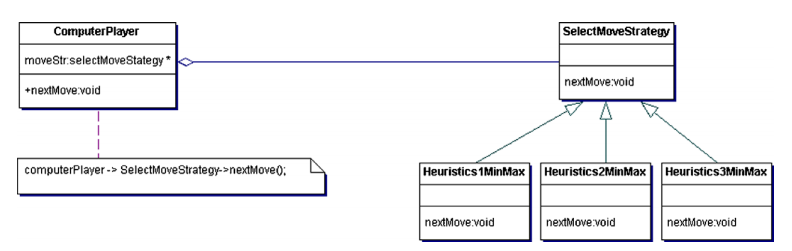
\includegraphics[width=\textwidth]{pics/strategypattern.png}
      \end{figure}

      {\bf Observer Pattern:} the observer pattern defines a one-to-many dependency between objects that when one objects changes state, all its dependants are notified and updated automatically. This can be used in a situation where a football manager game a team hires a trainer that upgrade players attributes.

      \begin{figure}[H]
        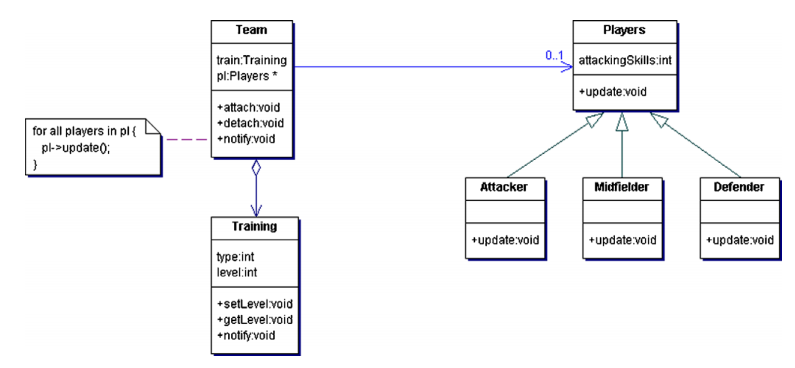
\includegraphics[width=\textwidth]{pics/observerpattern.png}
      \end{figure}

    \subsubsection*{Object-Oriented design patterns in GAME GRAPHICS}

    {\bf State Pattern:} the state pattern allows an object to alter it behaviour when its internal state change. This pattern can be used in games where an object changes the level of detail (LOD) of it apperance with respect of its distance from the camera. Feks a first person shooter, all objects of a scene should look more elegant as the main character reaches them. 

      \begin{figure}[H]
        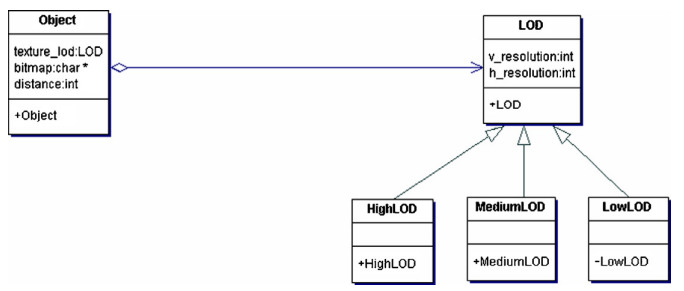
\includegraphics[width=\textwidth]{pics/statepattern.png}
      \end{figure}

    {\bf Bridge Pattern:} the bridge pattern decpuples an abstraction from its implementation so that the two can vary independently. This pattern can be used in any game with 3D objects that can be painted multiple ways. At the same time the 3D object might also vary since it can be a primitive (sphere, cube, etc) or an export from a 3D package. 

      \begin{figure}[H]
        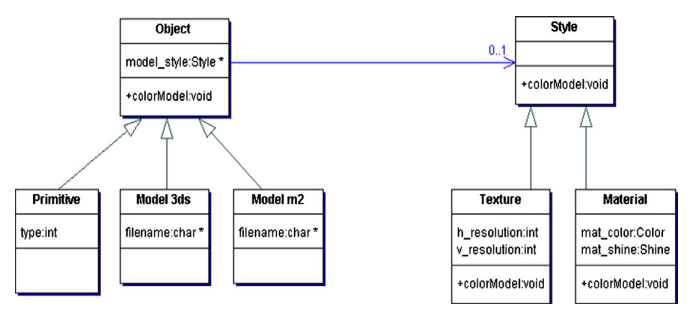
\includegraphics[width=\textwidth]{pics/bridgepattern.png}
      \end{figure}

  \section*{Evaluation}

    \subsubsection*{Software quality metrics}
    The software metrics that have been calculated can be divided into four main categories: size, complexity, coupling, and cohesion. 
    Coupling reduces the dependencies in calasses. 

      \begin{itemize}
        \item Lines of Code (LOC)
        \item Number of classes (NOC)
        \item Attribute Complexity (AC)
        \item Weighted Methods per Class 1 and 2 (WMPC1 and WMPC2)
        \item Cyclomatic Complexity (CC), number of possible paths.
        \item Coupling Factors (CF)
        \item Lack of Cohesion of Methods (LCOM)
      \end{itemize}

    \subsubsection*{Evaluation Example 1 - Cannon Smash}
    The drawback in the presented approach is that the incoming data could be recieved in three different types and according to the current type a different reading strategy should be used. In the first version the programmers used a switch statement to implement this mechanism. This code suffers from needless repitation. This code is not reuseable, because the program is not flexible enough to easily adapt the extra strategies. 

    A possible solution would be to use the strategy patten and in this way the complexity of the model will be decreased wheras the flexibility will increase. Attribute Complexity (AC) increased, Coupling decreased. Maintainable code. 

    \subsubsection*{Evaluation Example 2 - Ice Hockey Manager}
    Ice Hockey Manager is a simulation of coaching a hockey team. In the first version they used 8 design patterns. In a later version 26 design patterns was implemented, where bridge and state was two of the patterns used. 

    The state pattern represent the fact that a hockey player can either be a goalkeeper or a field player. This way, ant client of the program can create or handle a player without having to know in prior whether he is a goalkeeper or a field player. 

    The bridge pattern is used in order to provide a link between player an the player attributes interfaces so that the implementation of class player can be configured at run-time. 
    




\end{document}